%---------------------------------------------------------------------------------------------------
%		introduction.tex
%
%	This is file contains an introduction about the SOA architectural desing.
%
%	Author: Andrea Meneghinello
% Version: 0.1
%	Table of changes:
%		21/03/2016 -> document definition
%---------------------------------------------------------------------------------------------------
\section{\acf{soa}}
\label{sec:architecture-soa}
A \acf{soa} is an architectural model for the creation of systems that reside over a network and
focus their attention over the concept of \keyword{services}. A system built following the \ac{soa}
philosophy is made of applications called services. They are well defined, independent from each
other and they can reside on multiple computers linked in a network.

Each service makes a certain functionality available, and can utilize the ones made available by other
services. Though this architecture, we are able to build more sophisticated applications starting from
elementary components.

\ac{soa} is a particular form of distributed system, which definition: (comes from \cite{distributedSystem})

\begin{center}
	\begin{quote}
		``A distributed system consists of diverse, discrete software agents that must work together to perform
		some tasks. Furthermore, the agents in a distributed system do not operate in the same processing
		environment, so they must communicate by hardware/software protocol stacks over a network. This
		means that communications with a distributed system are intrinsically less fast and reliable than
		those using direct code invocation and shared memory. This has important architectural implications
		because distributed systems require that developers (of infrastructure and applications) consider
		the unpredictable latency of remote access, and take into account issues of concurrency and the
		possibility of partial failures.''
	\end{quote}
\end{center}

\subsection{Characteristics}
\label{sec:architecture-soa-characteristics}
\ac{soa} abstraction is not related to any specific technology, but it simply defines some properties 
that are oriented to the \keyword{reuse} and to the \keyword{integration} in a heterogeneous environments
of its base components.

In particular, each service must have the following properties (illustrated in Figure 
\ref{img:architecture-soa-characteristics}):

\begin{itemize}
	\item{\keyword{service discoverability}: a service must be retrieved basing on its interface and
		called at run-time;}
	\item{\keyword{service autonomy}: every service must be well defined, complete and independent
		from the context or from the status of other services;}
	\item{\keyword{standardized service contract} and \keyword{service abstraction}: services must
		be defined in terms of what they do, abstracting them from the technologies used to implement
		them. This determines the independence from both the used programming language and the \acs{os}
		on which they are running. It is not necessary to know how a service is implemented but only
		the offered functionalities.}
	\item{\keyword{service loose coupling}: an architecture is loosely coupled if the dependencies
		between its components are limited. Thus, we have to made services that depends least as possible
		by other making the system flexible and easily customizable;}
	\item{\keyword{service reusability}: each service must be made available on the network through
		the publication of its interface and made accessible in a transparent way (location awareness);}
	\item{\keyword{service statelessness}: the services minimize the resource consumption and delegate
		the status information management when necessary;}
	\item{\keyword{service composability}: in a \ac{soa} architecture the applications are the result of
		the composition of many services. This is the reason that leads us to build independent services
		in order to obtain the maximum re-usability. The creation of applications or more complex
		services through composability is defined as \keyword{service orchestration}.}
\end{itemize}

\begin{figure}
	\centering{}
	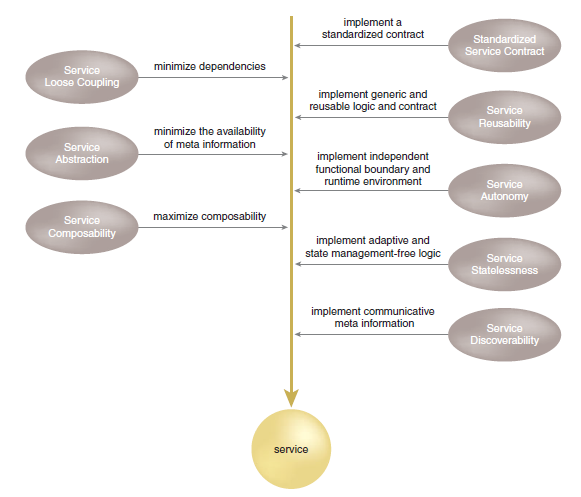
\includegraphics[width=0.7\textwidth]{chapters/architecture/images/soa-characteristics.png}
	\caption[Service oriented logic]{Service oriented logic \cite{serviceCharacteristics}.}
	\label{img:architecture-soa-characteristics}
\end{figure}

\subsection{How does \acs{soa} works}
\label{sec:architecture-soa-workmodel}
We can assert that there are three main actors in a \ac{soa} architecture. They are: \keyword{service
provider}, \keyword{service consumer} and \keyword{service registry}.

The service provider is the one responsible to provide service instances to other services. To make
them findable by other entities, they must be visible on the network, so they must be
\keyword{publicized}. During the publication phase, the service provider communicate to service registry
information about the service in order to memorize it. Then, the service registry contains all the
necessary information to access the service. When a consumer have to utilize the service instance, it
will made a request to the registry to know the necessary information in order to access it. In Figure
\ref{img:architecture-soa-workmodel} the interactions between the entity of the model are reported.

\begin{figure}
	\centering{}
	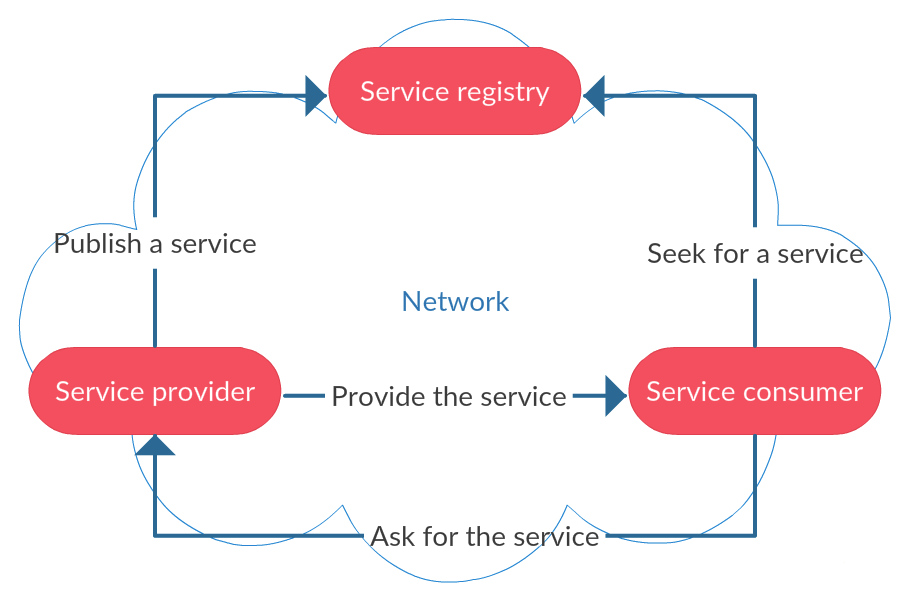
\includegraphics[width=0.7\textwidth]{chapters/architecture/images/soa-workmodel.png}
	\caption[Example of \acs{SOA} architecture]{Example of \acf{soa} architecture.}
	\label{img:architecture-soa-workmodel}
\end{figure}

All the interactions pass through network, which in a real scenario can be either Internet or a Intranet.
\ac{soa} defines the characteristics that the system components must have in order to
define the last one as a service-oriented architecture.

\subsection{Compatibility with cloud computing}
\label{sec:architecture-soa-compatibility}
\ac{soa} architecture is born in the pre-cloud era, thus it is not conceived to address cloud computing
issues. But \ac{caa} and \ac{soa} share some characteristics that bring us to consider \ac{soa}'s base
philosophy while building our architecture.

First, both emphasize the \keyword{service concept}. By definition, a service is made up by smaller parts
that do the job to build the final output, everyone use the \keyword{delegation} system. With that methodology,
people can use the services without worrying about their implementation details and scalability. Most
important, services can be shared by multiple applications and users, thus optimizing resource consumption.

Second, both promote the \keyword{loose} coupling concept principle. Each architecture demands minimum
dependencies among different parts of the system. As a result, any single change on one part of the system
has limited impact on the overall system.

Since \ac{soa} is born in the pre-cloud era it presents some differences that bring us to reconsider its
base philosophy before starting its adoption inside the cloud model. Both differ in term of
\keyword{horizontal and vertical services} and \keyword{applications vs. infrastructure}.

The services in \ac{soa} mainly focus on business. Each service may represent one aspect of the business.
Combined together, these services consist of a business application or solution. In this sense, the 
\keyword{services are horizontal}. Instead, the services in \ac{caa} are mainly layered according to 
typical software stacks. The lower services support the upper services to deliver applications. Therefore,
we call them \keyword{vertical services}.

\ac{soa} is for application architectures. The dividing of different components is based on their roles in
the \ac{soa} applications. More often than not, we start with a business problem and then abstract out the
services. These services can be re-used by other applications in the future. Instead cloud computing is for
\acs{it} delivery, so the dividing of different services is based on their roles in a software stack that is
mostly well defined. We do not need a problem before defining the cloud services. Services can be easily
re-used by every applications.

In conclusion, \ac{soa} and cloud computing share many common principles, but also differ significantly
in their role in \acs{it} architecture. \ac{soa} is mainly an application architecture with horizontal
services; while cloud computing is an \acs{it} architecture with vertical services. \ac{soa} played an
important role in cloud computing foundation. The service orientation paradigm supplies the \ac{saas}
provider with the necessary support for the implementation of interoperable services which can be flexibly
distributed and scaled as needed. The \ac{soa} concept allows cloud providers to adapt more quickly to
challenges of business. On the other hand, cloud computing is about providing ease of access to and usage of
services \cite{zuccato2014implementing}.

In following section we will explain a possible re-visitation of the \ac{soa}'s base principle making it more
suitable with the cloud computing definition.